\titre{\'Etude d'un domaine de $\R^2$}
\theme{topologie}
\auteur{}
\organisation{AMSCC}

Soit $D = \{(x,y) \in \R^2 \, , \, y \geq 0 \, , \, x-y > 0\}$ un domaine de $\R^2$.  
\begin{enumerate}
	\item Donner une représentation graphique de $D$. 
	\reponse{ 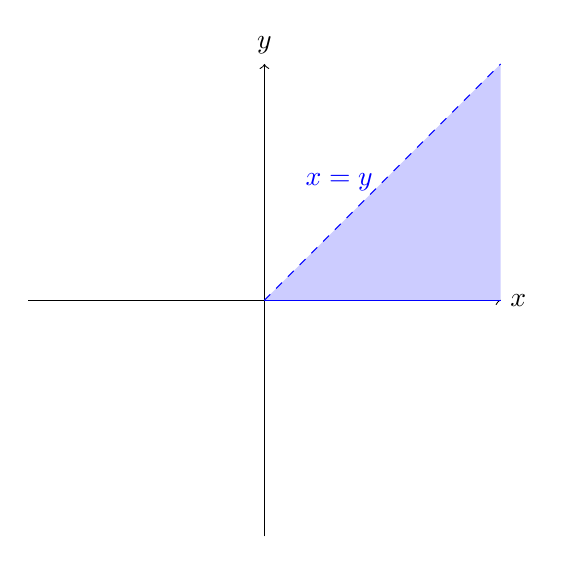
\begin{tikzpicture}[scale=1.5]
			\draw[->] (-2,0) -- (2,0) node[right] {$x$};
			\draw[->] (0,-2) -- (0,2) node[above] {$y$};
			\fill[blue!20,domain=0:2,smooth] (2,2) -- (2,0) -- (0,0) -- cycle;
			\draw[dashed, blue] (0,0) -- (2,2) node[midway,left] {$x=y$};
			\draw[blue] (0,0) -- (2,0);
		\end{tikzpicture}
	 }
	\item $D$ est-il ouvert dans $\R^2$ ? justifier rapidement. 
	\reponse{ $D$ n'est pas ouvert dans $\R^2$ car par exemple, le point $(1,0)$ appartient à $D$ mais aucune boule centrée en ce point de peut être contenue dans $D$. }
	\item $D$ est-il fermé dans $\R^2$ ? justifier rapidement. 
	\reponse{ $D$ n'est pas fermé dans $\R^2$ car par exemple, le point $(2,2)$ appartient au complémentaire de $D$ et aucune boule centrée en ce point ne peut être contenue dans le complémentaire de $D$. }
	\item Vérifier que le point $(2,2)$ n'appartient pas à $D$ mais qu'en revanche, il existe une suite de points $(x_n,y_n) \in D$ tels que $(x_n,y_n) \xrightarrow[n \to +\infty]{} (2,2)$.
	\reponse{ On a $2-2 = 0$ donc $(2,2) \notin D$, en revanche on peut définir la suite $(x_k,y_k) = (2+1/k,2-1/^k) \in D$ qui converge vers $(2,2)$. }
\end{enumerate}